\documentclass[journal=esthag,manuscript=article]{achemso}

% additional packages
\usepackage[utf8]{inputenc}
\usepackage{amsmath}
\usepackage{booktabs}
\usepackage{subcaption}
\usepackage{tabularx}
\usepackage{array,multirow,graphicx}
\usepackage{comment}
\graphicspath{
  {./../figures/},
  {./../figures/2d_kde/},
  {./../figures/simulation_predictions/},
  {./../figures/pair_grids/},
  {./../figures/temporal_variability/},
}
\usepackage{lineno}
\linenumbers
% macros

% authors
\author{Jonathan G. V. Ström}
\affiliation[Brown University]{Brown University, School of Engineering, Providence, RI, USA}
\author{Yijun Yao}
\affiliation[Zhejiang University]{Zhejiang University, Hangzhou, China}
\author{Eric M. Suuberg}
\email{eric_suuberg@brown.edu}
\affiliation[Brown University]{Brown University, School of Engineering, Providence, RI, USA}

% title
\title{Transient Variability In Vapor Intrusion And The Factors That Influence It}

% keywords
\abbreviations{VI}
\keywords{Vapor intrusion, Preferential pathways, Temporal variability, Factor analysis, Modeling}

\begin{document}

\begin{abstract}

\end{abstract}

\section{Introduction}

Long term vapor intrusion (VI) studies in both residential and larger commercial structures have raised concerns regarding significant observed transient behavior in indoor air contaminant concentrations\cite{u.s._environmental_protection_agency_oswer_2015,folkes_observed_2009,holton_temporal_2013,johnston_spatiotemporal_2014,hosangadi_high-frequency_2017,mchugh_recent_2017,u.s._environmental_protection_agency_assessment_2015}.
VI involves the migration of volatilizing contaminants from soil, groundwater or other subsurface sources into overlying structures. VI has been a recognized problem for some time, but many aspects remain poorly understood, particularly with respect to the causes of large temporal transients in indoor air concentrations.
There is uncertainty within the VI community regarding how to best develop sampling strategies to address this problem\cite{u.s._environmental_protection_agency_oswer_2015,holton_temporal_2013,johnson_integrated_2016}. \par

Results from a house operated by Arizona State University (ASU) near Hill AFB in Utah, an EPA experimental house in Indianapolis, IN and a large warehouse at the Naval Air Station (NAS) North Island, CA have all shown significant transient variations in indoor air contaminant concentrations.
All were outfitted with sampling and monitoring equipment that allowed tracking temporal variation in indoor air contaminant concentrations on time scales of hours.
All have shown that these concentrations varied significantly with time - orders of magnitude on the timescale of a day or days.
\cite{holton_evaluation_2015,guo_vapor_2015,hosangadi_high-frequency_2017}. \par

In one instance the source of the variation was clearly established during the study; at the ASU house a field drain pipe (or “land drain”), which connected to a sewer system, was discovered beneath the house, and careful isolation of this source led to a clear conclusion that this preferential pathway significantly contributed to observed indoor air contaminant levels and their fluctuations\cite{guo_vapor_2015,guo_identification_2015}.
While in this case the issue of a contribution from a preferential pathway was clearly resolved, what it left open was a question of whether existence of such a preferential pathway to an area beneath a structure would always be expected to lead to large fluctuations in indoor air contaminant concentrations. \par

Similarly, a sewer pipe has recently been suggested to be a source of the contaminants found in the EPA Indianapolis house.
That site was also characterized by large indoor air contaminant concentration fluctuations\cite{mchugh_evidence_2017,u.s._environmental_protection_agency_assessment_2015}.
Sewer lines have been generally implicated as VI sources at several sites\cite{pennell_sewer_2013,mchugh_evidence_2017,roghani_occurrence_2018,riis_vapor_2010}.
A Danish study estimate that roughly 20\% of all VI sites in central Denmark involve significant sewer VI pathways\cite{nielsen_remediation_2017}.
Thus while the consideration of a role of possible sewer or other preferential pathways is now part of normal good practice in VI site investigation\cite{u.s._environmental_protection_agency_oswer_2015}, it is still not known whether the existence of such pathways automatically means that large temporal fluctuations are necessarily to be expected.
In some of these cited cases\cite{pennell_sewer_2013,riis_vapor_2010}, a sewer provided a pathway for direct entry of contaminant into the living space.
While potentially important in many cases, this scenario is not further considered here, where the focus is on pathways that deliver contaminant via the soil beneath a structure. \par

It is, however, now known that even absent a preferential pathway, there may be significant transient variation in indoor air contaminant concentrations at VI sites\cite{folkes_observed_2009,brenner_results_2010,johnston_spatiotemporal_2014}.
One example is a site at NAS North Island at which no preferential pathways have been identified.
Instead, a building at this site is characterized by significant temporal variations in indoor-outdoor pressure differential\cite{hosangadi_high-frequency_2017}.
It is believed that this is the origin of the observed indoor air contaminant concentration fluctuations at that site. \par

This paper investigates the sources of the temporal variation in indoor air contaminant concentrations in both the presence and absence of preferential pathways.
In this work, the latter scenarios are referred to as ”normal” VI scenarios, in which there is typically a groundwater source of the contaminant.
Specifically, we pose the question of just how much variation in indoor air contaminant concentration may be expected at  such normal  VI  sites vs. those characterized by preferential pathways.
The conditions required for preferential pathways to become significant contributors to temporal variations in indoor air contaminant concentrations are also explored, and the consequences for sampling strategies are also discussed.



\section{Methods}


\subsection{Statistical Analysis Of Field Data}

To begin to characterize transient behavior in indoor air contaminant concentrations, actual datasets are analyzed to establish common levels of variability at VI sites.
For this purpose, the datasets from the ASU house in Utah, the EPA Indianapolis site and North Island NAS were chosen for analysis.
This paper relies on statistical analysis of published field data, and readers are referred to the original works for details regarding data acquisition\cite{holton_evaluation_2015,guo_vapor_2015,holton_temporal_2013,hosangadi_high-frequency_2017,u.s._environmental_protection_agency_assessment_2015}. \par

The ASU house data were obtained over a period of a few years.
During part of this time, controlled pressure method (CPM) tests were being conducted, in which the house was underpressurized to an extent greater than that characterizing “normal” operation.
This caused greater than normal advective flow from the subsurface into the house, thus increasing VI potential\cite{mchugh_evaluation_2012,mchugh_recent_2017,holton_evaluation_2015}.
This period of CPM testing is considered separately from the otherwise ”natural” VI conditions in the analysis.
Likewise, the existence of a preferential pathway at the ASU house needs to be considered in examining the dataset, noting that during some of the testing, this pathway was deliberately cut off, resulting in what we have termed “normal” VI conditions in which the main source of contaminant was believed to be groundwater. \par

The NAS North Island dataset has not (as far as is known) been influenced by a preferential pathway, but the structure there was subject to large internal pressure fluctuations, much more extensive than those typically recorded at the ASU house during normal operations.
Additionally, the underlying soil at NAS North Island is sandy and more permeable than that at the ASU site, which, as will be shown, contributes to the indoor air contaminant concentrations being more sensitive to pressure fluctuations\cite{hosangadi_high-frequency_2017}. \par

Likewise, the Indianapolis site investigation spanned a number of years and periodically included the testing of a sub-slab depressurziation system (SSD).
The goal of the SSD testing was to mitigate the VI risk by drastically depressurizing the sub-slab area underneath the house, preventing the contaminants from entering the structure above.
Only the period before the installation of this system was considered in the present analysis.
It is likely a sewer line beneath the structure acted as a preferential pathway\cite{mchugh_evidence_2017}, however at no point was this preferential pathway removed, making it difficult to assess how significant the role of the preferential pathway was at this site.
Regardless of this it is of interest to consider the data from this site due to how extensive and complete the data collection was. \par

The typical variation in indoor air contaminant concentrations with time will first be considered below in the case of the ASU house during ”natural”, (i.e. non-CPM conditions), in the case of the NAS North Island site over the entire available dataset, and for the Indianapolis case we consider the variations before the installation of the SSD system.
The deviations in indoor air concentration from the mean TCE (and Chloroform and PCE at the Indianapolis site) values, as well as the indoor-outdoor pressure differentials associated with these concentrations were examined.
Both univariate and bivariate kernel density estimations (KDE) were constructed.
KDE is a technique that estimates the probability distribution of a random variable(s) by using multiple kernels, or weighting functions, and in this case, Gaussian kernels are used to create the KDEs.
This means that it is presumed that the variables of interest (i.e., indoor air contaminant concentrations and indoor-outdoor pressure differentials, as sampled) are normally distributed around mean values (and that there are statistical fluctuations associated with each sampling event).
In this instance, the scipy statistical package was used to construct the KDEs, assuming a bandwidth parameter determined by Scott's rule.
The distributions of the individual parameters and the relationship between them will be examined using the KDE method.

\subsection{Modeling Work}
In addition to examining the actual field data, a previously described three -dimensional computational fluid dynamics model of a generic VI impacted house was used to elucidate certain aspects of  the processes.
This model was implemented in a finite element solver package, COMSOL Multiphysics.
In the present work, there has been an addition of a preferential pathway to the ”standard” model that has been described before in publications by this group\cite{shen_influence_2013,yao_investigating_2017,yao_three-dimensional_2017}.
As in the earlier studies, only the vadose zone soil domain is directly modeled.

The modeled structure is assumed to have a 10x10 m foundation footprint, with the bottom of the foundation slab lying 1 m below ground surface (bgs), simulating a house with a basement.
The indoor air space is modeled as a continuously stirred tank (CST)\cite{u.s._environmental_protection_agency_oswer_2015} and all of the contaminant entering the house is assumed to enter with soil gas through a 1 cm wide crack located between the foundation walls and the foundation slab around the perimeter of the house.
All of the contaminant leaving the indoor air space is assumed to do so via air exchange with the ambient.
The indoor control volume is assumed to consist of only of the basement, assumed as having a total volume of $300 \; \mathrm{m^3}$.
Clearly different assumptions could be made regarding the structural features and the size of the crack entry route, but for present purposes, this is unimportant as the intent is only to show for “typical” values what the influence of certain other features can be. \par

The modeled surrounding soil domain extends 5 meters from the perimeter of the house, and is assumed to consist of sandy clay (except as noted).
Directly beneath the foundation slab, there is assumed to be a 30 cm (one foot) thick gravel layer, except in certain cases where this sub-base material is assumed to be the same as the surrounding soil (termed  a ”uniform” soil scenario). \par

Where relevant The preferential pathway is modeled as a 10 cm (4”) pipe that exits into the gravel sub-base beneath the structure.
The air in the pipe is assumed to be contaminated with TCE at a vapor concentration equal to the vapor in equilibrium with the groundwater contaminant concentration below the structure, modified by a scaling factor $\chi$, allowing the contaminant concentration in the pipe to be parameterized. \par

The groundwater beneath the structure is assumed to be homogeneously contaminated with trichloroethylene (TCE) as a prototypical contaminant.
The groundwater itself is not modeled, as the bottom of the model domain is defined by the top of the water table.
The ground surface and the pipe are both assumed to be sources of air to the soil domain.
Both are assumed to be at reference atmospheric pressure. \par

Vapor transport in the soil is governed by Richard’s equation, a modified version  of Darcy’s Law, taking the variability of soil moisture in the vadose zone into account\cite{richards_capillary_1931}.
The van Genuchten equations are used to predict the soil moisture content and thus the effective permeability of the soil\cite{van_genuchten_closed-form_1980}.
The effective diffusivity of contaminant in soil is calculated using the Millington-Quirk model\cite{millington_permeability_1961}.
The transport of vapor contaminant in the soil is assumed to be governed by the advection-diffusion equation, in which either advection or diffusion may dominate depending upon position and particular circumstances.
The equations and the boundary conditions are given in Table \ref{tbl:eqns-bc-parameters}.

\begin{table}[htb!]
  \centering
  \caption{Governing equations, boundary conditions \& model input parameters. (See below for table of nomenclature).}
  \label{tbl:eqns-bc-parameters}
  \bigskip
  %%%%%%%%%%%%%%%%%%%%%%%%%%%%%%%%%%%%%%%%%%%%%%%%%%%%%%%%%%%%%%%%%%%%%%%%%%%%%%
  % Governing equations
  %%%%%%%%%%%%%%%%%%%%%%%%%%%%%%%%%%%%%%%%%%%%%%%%%%%%%%%%%%%%%%%%%%%%%%%%%%%%%%
  \subcaption{Governing equations}
  \begin{tabular}{l l}
    \toprule
    % Indoor air space equation
    Unsteady-CSTR                 & $V\frac{d u}{d t} = \int_{A_\mathrm{ck}} j_\mathrm{ck} dA - u A_e V$ \\
    % Richard's equation
    Richard's equation            & $\nabla \cdot \rho \Big( - \frac{\kappa_s}{\mu} k_r \nabla p \Big) = 0$ \\
    % Millington-Quirk equation
    Millington-Quirk              & $D_\mathrm{eff} = D_\mathrm{air}\frac{\theta_g^{10/3}}{\theta_t^2} + \frac{D_\mathrm{water}}{K_H} \frac{\theta_w^{10/3}}{\theta_t^2}$ \\
    % Advection-diffusion equation
    Advection-diffusion equation  & $\frac{\partial}{\partial t} \Big( \theta_w c_w + \theta_g c \Big) = \nabla (D_\mathrm{eff} \cdot \nabla c) - \vec{u} \cdot \nabla c$ \\
    % van Genuchten's equations
    \multirow{3}{*}{van Genuchten equations}     & $\mathrm{Se} = \frac{\theta_w - \theta_r}{\theta_t - \theta_r} = [1 + |\alpha z|^n]^{-m}$ \\
                                  & $\theta_g = \theta_t - \theta_w$ \\
                                  & $k_r = (1 - \mathrm{Se})^{l} [1 - (\mathrm{Se}^{-m})^m]^2$ \\
                                  & $m = 1 - 1/n$ \\
    \bottomrule
  \end{tabular}
  \bigskip
  %%%%%%%%%%%%%%%%%%%%%%%%%%%%%%%%%%%%%%%%%%%%%%%%%%%%%%%%%%%%%%%%%%%%%%%%%%%%%%
  % Boundary conditions
  %%%%%%%%%%%%%%%%%%%%%%%%%%%%%%%%%%%%%%%%%%%%%%%%%%%%%%%%%%%%%%%%%%%%%%%%%%%%%%
  \subcaption{Boundary conditions}
  \begin{tabular}{l l l}
    \toprule
    \textbf{Boundary}          & \textbf{Richard's equation}      &   \textbf{Advection-diffusion equation} \\
    % Foundation crack
    At foundation crack  & $p = p_\mathrm{in/out} \; \mathrm{(Pa)}$                            & $j_\mathrm{ck} = \frac{u c}{1 - \exp{(u L_\mathrm{slab}/D_\mathrm{air})}}$ \\
    % Groundwater source
    At groundwater source &  N/A & $c = c_\mathrm{gw} K_H \; \mathrm{(\mu g/m^3)}$ \\
    % Ground surface
    At ground surface      & $p = 0 \; \mathrm{(Pa)}$  & $c = 0 \; \mathrm{(\mu g/m^3)}$ \\
    % Preferential pathway
    Exit of preferential pathway  & $p = 0 \; \mathrm{(Pa)}$  & $c = c_\mathrm{gw} K_H \chi \; \mathrm{(\mu g/m^3)}$ \\
    \bottomrule
  \end{tabular}
  \bigskip
  %%%%%%%%%%%%%%%%%%%%%%%%%%%%%%%%%%%%%%%%%%%%%%%%%%%%%%%%%%%%%%%%%%%%%%%%%%%%%%
  % Soil input parameters
  %%%%%%%%%%%%%%%%%%%%%%%%%%%%%%%%%%%%%%%%%%%%%%%%%%%%%%%%%%%%%%%%%%%%%%%%%%%%%%
  \subcaption{Soil \& gravel properties\cite{dan_capillary_2012,abreu_conceptual_2012,u.s._environmental_protection_agency_userss_2004}}
  \begin{tabular}{l l l l l l l}
    \toprule
    % Descriptions
    Soil & $\text{Permeability} \; \mathrm{(m^2)}$  & $\mathrm{Density} \; \mathrm{(kg/m^3)}$  & $\theta_s$  & $\theta_r$  & $\alpha \; \mathrm{(1/m)}$  & $n$ \\
    % Gravel
    Gravel     & $1.3 \cdot 10^{-9}$   & 1680    & 0.42        & 0.005       & 100       & 3.1 \\
    % Sand
    Sand     & $9.9 \cdot 10^{-12}$  & 1430    & 0.38        & 0.053        & 3.5       & 3.2 \\
    % Sandy clay
    Sandy Clay    & $1.7 \cdot 10^{-14}$  & 1470    & 0.39        & 0.12        & 3.3       & 1.2 \\
    \bottomrule
  \end{tabular}
  \bigskip
  %%%%%%%%%%%%%%%%%%%%%%%%%%%%%%%%%%%%%%%%%%%%%%%%%%%%%%%%%%%%%%%%%%%%%%%%%%%%%%
  % TCE input parameters
  %%%%%%%%%%%%%%%%%%%%%%%%%%%%%%%%%%%%%%%%%%%%%%%%%%%%%%%%%%%%%%%%%%%%%%%%%%%%%%
  \subcaption{Trichloroethylene (diluted in air) properties\cite{abreu_conceptual_2012,u.s._environmental_protection_agency_userss_2004}}
  \begin{tabular}{l l l l l l}
    \toprule
    $D_\mathrm{air} \; \mathrm{(m^2/h)}$  & $D_\mathrm{water} \; \mathrm{(m^2/h)}$  & $\mathrm{Density} \; \mathrm{(kg/m^3)}$ & $\mathrm{Viscosity} \; \mathrm{(Pa \cdot s)}$  & $K_H$ & $M \; \mathrm{(g/mol)}$ \\
    $2.47 \cdot 10^{-2}$  & $3.67 \cdot 10^{-6}$  & 1.614 & $1.86 \cdot 10^{-5}$  & 0.403 & 131.39 \\
    \bottomrule
  \end{tabular}
  \bigskip
  %%%%%%%%%%%%%%%%%%%%%%%%%%%%%%%%%%%%%%%%%%%%%%%%%%%%%%%%%%%%%%%%%%%%%%%%%%%%%%
  % Building input parameters
  %%%%%%%%%%%%%%%%%%%%%%%%%%%%%%%%%%%%%%%%%%%%%%%%%%%%%%%%%%%%%%%%%%%%%%%%%%%%%%
  \subcaption{Building properties}
  \begin{tabular}{l l l}
    \toprule
    $V_\mathrm{base} \; \mathrm{(m^3)}$  & $L_\mathrm{slab} \; \mathrm{(cm)}$  & $A_e \; \mathrm{(1/hr)}$ \\
    %
    300  &  15  & 0.5 \\
    \bottomrule
  \end{tabular}
\end{table}

\section{Results \& Discussion}

\subsection{Statistical Analysis of Field Data}

\begin{figure}[htb!]
		\centering
    \caption{Distributions of indoor/outdoor pressure differences (top row), and its correlation with indoor air contaminant concentrations (middle rows), and air exchange rate (bottom row), at three different VI sites - ASU house, Indianapolis site, and North Island NAS.}
    \label{fig:kde}
    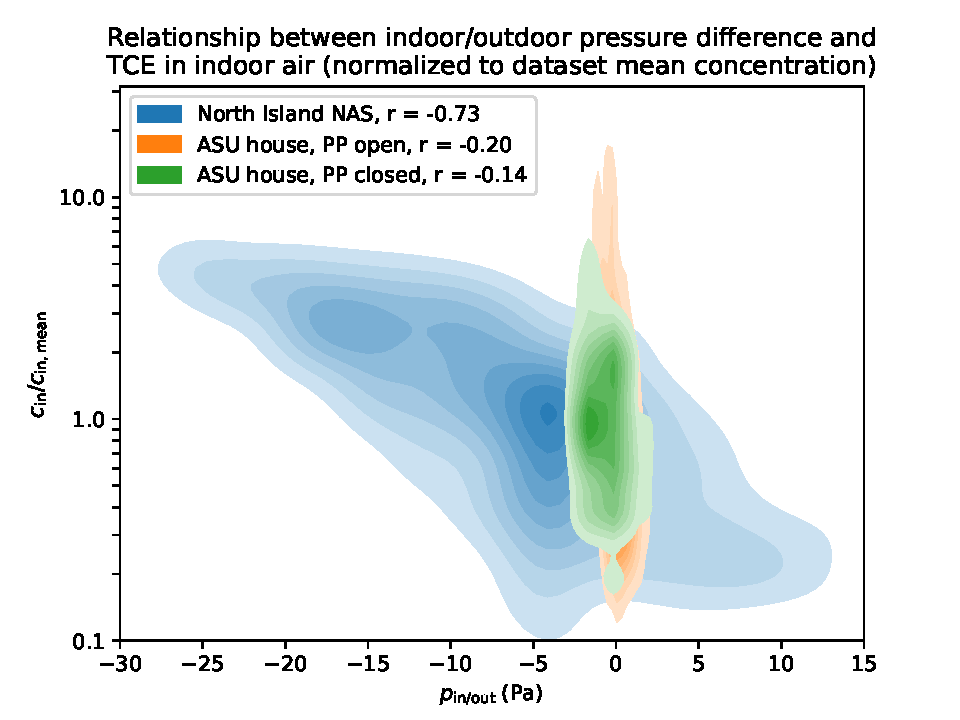
\includegraphics[width=\textwidth]{nas_asu_pp.pdf}
\end{figure}

\begin{table}[htb!]
  \caption{5th and 95th percentile values of $p_\mathrm{in/out}$ and $c_\mathrm{in}/c_\mathrm{in,mean}$ in Figure \ref{fig:kde}.}\label{tbl:percentiles}
  \begin{tabular}{c c c c c c c}
    \toprule
    & \multicolumn{2}{c|}{\textbf{North Island NAS}} & \multicolumn{2}{c|}{\textbf{ASU house PP Open}} & \multicolumn{2}{c}{\textbf{ASU House PP Closed}} \\
    Percentile & 5th & 95th & 5th & 95th & 5th & 95th \\
    $p_\mathrm{in/out}$ (Pa) & -19.9 & 7.4 & -1.4 & 2.1 & -2.1 & 2.27 \\
    $c_\mathrm{in}/c_\mathrm{in,mean}$ & 4.1 & 0.2 & 13.5 & 0.2 & 3.3 & 0.4 \\
    \bottomrule
  \end{tabular}
\end{table}

The pressure difference between the indoor and outdoor/ambient ($p_\mathrm{in/out}$) is an important driving force in VI, drawing in (or preventing) contaminants from entering a structure. % TODO: Add references
Changes in $p_\mathrm{in/out}$ is also a dynamic and fast process, impacting VI more rapidly than e.g. fluctuations in groundwater depth or contaminant concentration does; these processes may take weeks or even months to impact the overlying structure.
Therefore it is reasonable to assume that the temporal variability in indoor air contaminant concentration $c_\mathrm{in}$ may be driven by changes in $p_\mathrm{in/out}$.

We examine the relationship between $p_\mathrm{in/out}$ and $c_\mathrm{in}$  by constructing the two-dimensional kernel density estimation (KDE) plots seen in Figure \ref{fig:kde}.
The KDE plot allows us to view the distribution of $p_\mathrm{in/out}$ and $c_\mathrm{in}$, and how well these correlate.
For this analysis we consider two VI sites, North Island NAS, and the ASU house, with the ASU house dataset divided up into two periods, before and after the land drain (called preferential pathway (PP) from here on) had been closed.
The preferential pathway significantly impacted the ASU house to such an extent that these two periods can essentially be considered as two different VI sites, and allowing us to examine the effect it had.

In Figure \ref{fig:kde} $c_\mathrm{in}$ is normalized to the mean $c_\mathrm{in,mean}$ of each dataset, allowing us to compare the impact $p_\mathrm{in/out}$ had on $c_\mathrm{in}$.
A value of 10 on the y-axis indicate that $c_\mathrm{in}$ is 10 times greater than the mean here, and 0.1 indicate that it is one tenth of the mean.
The Pearson's r between $p_\mathrm{in/out}$ and $c_\mathrm{in}$ for each dataset is shown in the legend.

An interesting aspect of the North Island NAS site is that $p_\mathrm{in/out}$ varies so significantly here, with the 5th and 9th percentile $p_\mathrm{in/out}$ -19.9 and 7.4 Pa respectively.
This may be contrasted with 5th and 95th percentile $p_\mathrm{in/out}$ at the ASU house: -1.4 and 2.1 Pa (PP open), and -2.1 and 2.27 Pa (PP closed).

The large (roughly one order of magnitude) under- and overpressurization of the North Island NAS site leads to roughly a one order magnitude increase and decrease from the mean $c_\mathrm{in}$.
Combined with $r=-0.73$, it is quite clear that at this site $p_\mathrm{in/out}$ largely determines $c_\mathrm{in}$ (there is still variability in $c_\mathrm{in}$ for a given $p_\mathrm{in/out}$, which we address later).
This is the same principle that governs the controlled pressure method (CPM) concept.

Turning to the ASU house datasets, we see a quite different situation.
Here the variability of $c_\mathrm{in}$ is just as large, or even larger than at North Island NAS, yet the $p_\mathrm{in/out}$ varies far less.
At first glance it may seem like the $c_\mathrm{in}$ values for the periods when the PP is open and closed respectively are relatively comparable, but the 5th and 95th percentiles values of differ significantly $c_\mathrm{in}/c_\mathrm{in,mean}$ as may be seen in Table \ref{tbl:percentiles}.

It is clear that the PP dramatically increases the house's sensitivity to $p_\mathrm{in/out}$, and the site is fundamentally different during the period when the PP was open.
Yet, the magnitude of change in $c_\mathrm{in}$ is far greater than the change in $p_\mathrm{in/out}$, leading to the conclusion that it is not just increased flow rates into the structure that causes this, but there must also be an increased amount of contaminant as well as a much larger spatial variability in the sub-base.
This is a topic that we will return to later.

The magnitude of change in $c_\mathrm{in}$ when the PP is closed is more in line with the magnitude of change in $p_\mathrm{in/out}$, but there is still more variability than one would expect.
We hypothesize that this is largely due to fluctuations in air exchange rate, which we will examine later.

\subsection{Change In Indoor Air Contaminant Concentration Over Time} % TODO: Improve title

\begin{figure}[htb!] % TODO: Adjust aspect ratio
  \centering
  \caption{ (1D is 1 day, 2W is 2 weeks, and 3M is 3 months).}
  \label{fig:resampling}
  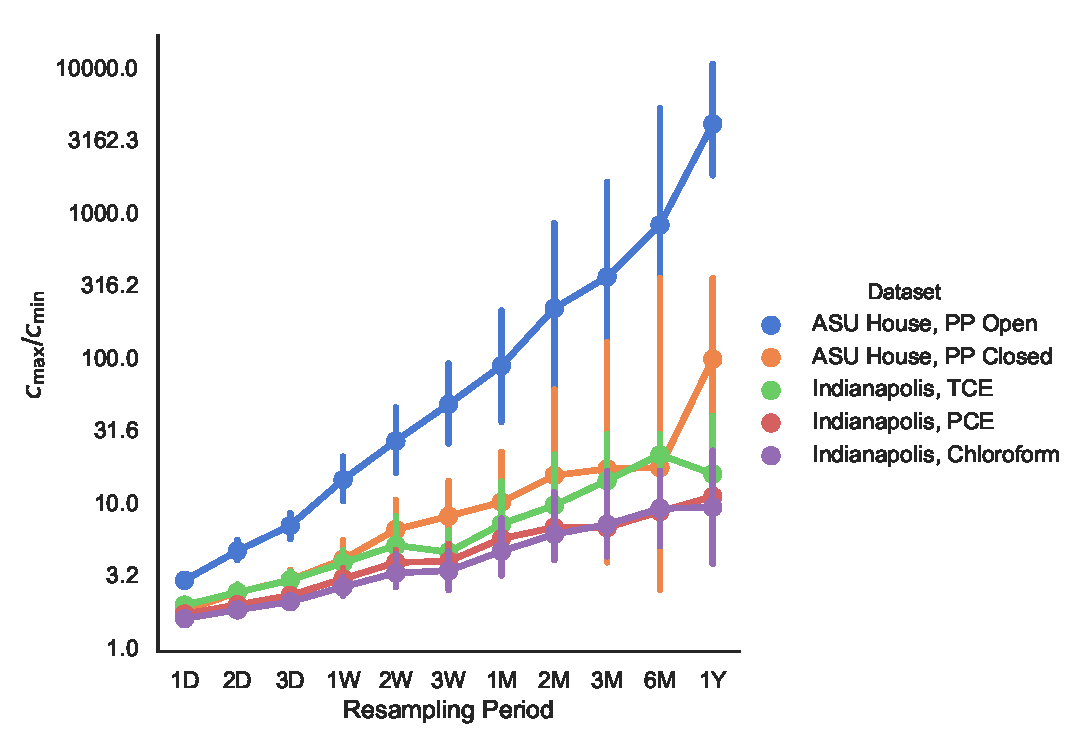
\includegraphics[width=\textwidth]{temporal_variability/resampling.pdf}
\end{figure}

% RESAMPLING TIME ANALYSIS
So far we have discussed how the relationship between $c_\mathrm{in}$ and $p_\mathrm{in/out}$, and how significantly $c_\mathrm{in}$ may vary at a site.
But this tells us little about how much variability in $c_\mathrm{in}$ may be expected over time.
For this analysis we turn to the ASU house data (PP open/closed considered separately again), and another well-studied VI site, the Indianapolis site in Indiana.
Both of these sites collected high frequency $c_\mathrm{in}$ samples over a significant periods and are therefore suitable. % TODO: Reference to the time periods here
Furthermore, at Indianapolis site the $c_\mathrm{in}$ of three different contaminants, Chloroform, Trichloroethylene (TCE), and Tetrachloroethylene (PCE) were collected, allowing us to see if there is any difference in the variability of each.
The North Island NAS dataset only spans a few days, and is therefore excluded from this analysis.

To demonstrate how significantly $c_\mathrm{in}$ can vary across time, we calculate at the quotient of the maximum and minimum $c_\mathrm{in}$ (denoted as $c_\mathrm{max}/c_\mathrm{min}$) over a given time period.
I.e. if $c_\mathrm{in}$ samples were collected every four hours over a period of a year, and the data is resampled on a daily basis, then $c_\mathrm{max}/c_\mathrm{min}$ is returned for within each day, giving 365 data points.
Resampling periods of one, two, three, days, weeks, and months are chosen and Figure \ref{fig:resampling} shows the result of this analysis.

As one might expect, the longer the resampling period, the larger the maximum variability is, spanning from less than a threefold difference, to two to three orders of magnitude.
That such a large variability is observed when the resampling time approaches the length of the entire datasets is hardly surprising, nor is it surprising that the variability is much more significant when the preferential pathway was open than closed.
What may be surprising is that absent a preferential pathway such as the one at the ASU house, it may take a few weeks before an order of magnitude maximum variability is reached.
The most significant result of this analysis is that the maximum variability is quite small across a few days, suggesting that e.g. 24-hour passive samplers will resolve the daily temporal variability in $c_\mathrm{in}$ well ($c_\mathrm{max}/c_\mathrm{min} \approx 1.5$) and that a sampling frequency greater than a few days may yield little extra information.
There is also little difference between maximum variability of $c_\mathrm{in}$ the ASU house (when the PP is closed), and the three contaminants at the Indianapolis site.

% ASU:
% Pressure distributions similar
% Yet drastically different c
% => clearly driven by PP
% Pressure relationship better when open than close
% => Enhanced advection, motivating our choice of model
% Poor relationship for closed,
% => Diffusion dominated transport
% Yet significant uncertainty and variance in indoor air?
% Look at the influence of Ae on this
% Pressure is related to Ae, but not determinant
% => still large variability in Ae for a given p, what effect does this have?

% Indianapolis & North Island
% Unforunately no Ae data here like ASU, cannot look at that influence
% Stronger correlation between p and c here
% Indianapolis had some type of PP, though less significant than at ASU
% North Island had very large pressure changes, may explain the stronger relationship

\subsubsection{Influence Of Pressure On Indoor Air Variability}


\begin{figure}[!h] % TODO: Adjust aspect ratio
	\centering
  \caption{Simulated cases}
  \label{fig:land_drain_scenarios_fluctuating_ae}
  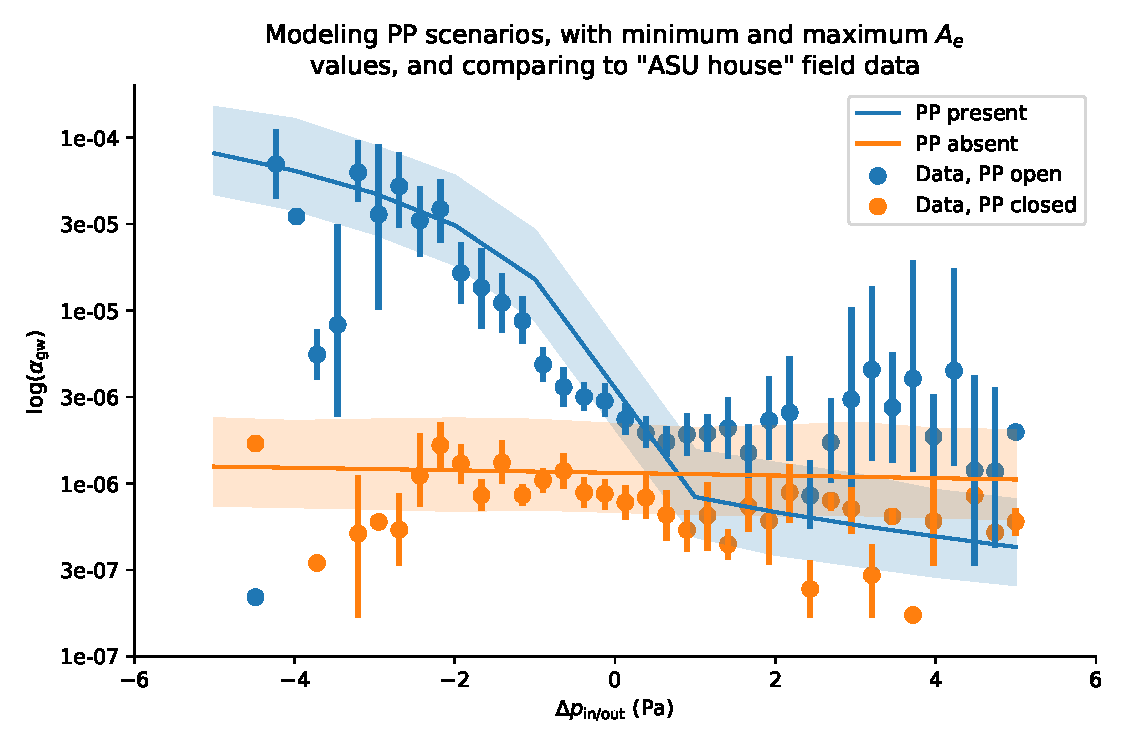
\includegraphics[width=\textwidth]{land_drain_scenarios_fluctuating_ae.pdf}
\end{figure}


\begin{comment}
\begin{figure}[!h] % TODO: Adjust aspect ratio
	\centering
  \caption{Simulated cases}
  \label{fig:land_drain_scenarios_constant_ae}
  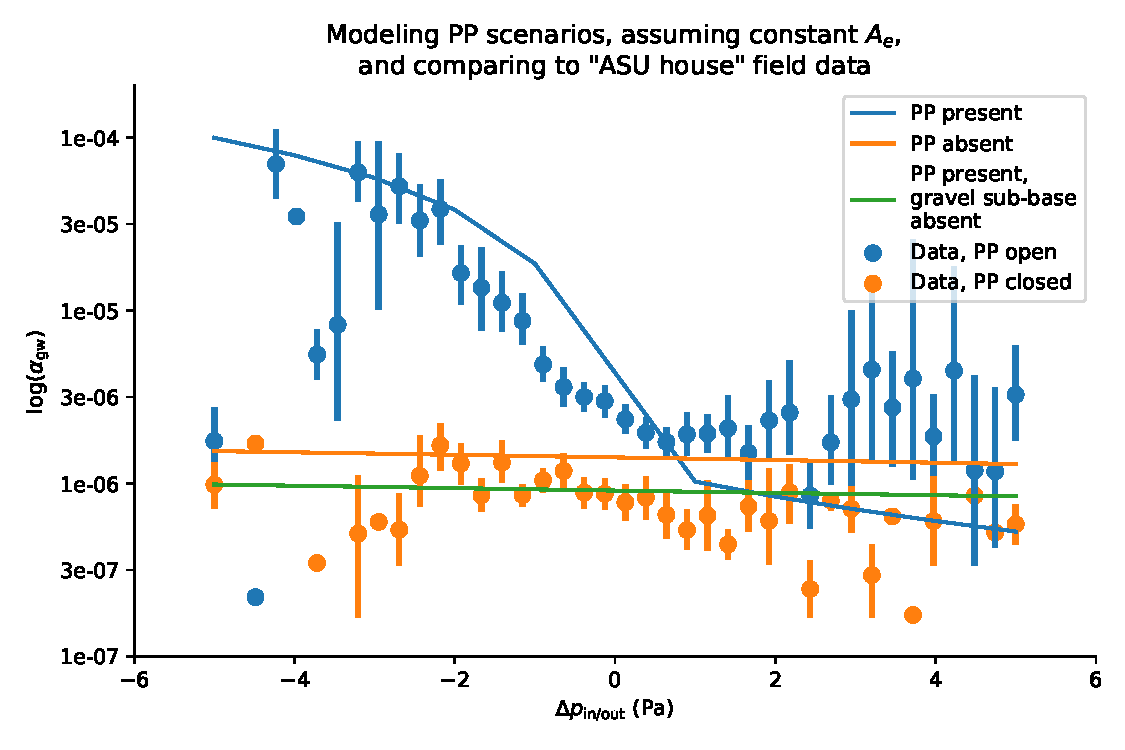
\includegraphics[width=0.5\textwidth]{land_drain_scenarios_constant_ae.pdf}
\end{figure}

To examine the role that $p_\mathrm{in/out}$ and $A_e$ play in determining $c_\mathrm{in}$ variability (given as attenuation from groundwater vapor source $\alpha_\mathrm{gw}$ here), we first consider modeling VI scenarios with a constant $A_e = 0.5 \; \mathrm{(1/hr)}$ (the mean $A_e$ at the ASU house), and varying $p_\mathrm{in/out}$ from 5 to -5 Pa.
The first of these scenarios is aimed to be similar to the period when the preferential pathway is open at the ASU house, and thus the modeled preferential pathway is active.
In the second scenario, this preferential pathway feature is deactivated, akin to the period when the preferential pathway was closed at the ASU site.
And in the third, the preferential pathway is again modeled, but the permeable gravel sub-base is instead assumed consist of the sandy loam, just like the surrounding soil, giving an "uniform soil" scenario. % TODO: Make sure that the soil type is correct
The results of these modeled scearios are then compared to the preferential pathways "open" and "closed" periods from the ASU data, and may be seen in Figure \ref{fig:land_drain_scenarios_constant_ae}.
The data is here binned into evenly spaced bins, with each dot representing the mean $\alpha_\mathrm{gw}$ and the error bars denote the one standard deviation.

By examining the first scenario (blue) it is readily apparent that the model is able to capture the behavior of the preferential pathway when the structure is depressized ($p_\mathrm{in/out} < 0$) but not very well when the house is overpressurized ($p_\mathrm{in/out} > 0$).
This shows that the preferential pathways acts by increasing advective potential, allowing even relatively small increases in depressurziation dramatically increases the contaminant entry rate into the house.
Conversely, when the structure is overpressurized, contaminant entry is more effectively inhibited, leading to diffusion being the more important transport mechanism from the sub-base to the indoor air space, leading to the decrease in $\alpha_\mathrm{gw}$.
Yet, when $p_\mathrm{in/out} > 0$ there is a slight increase in $\alpha_\mathrm{gw}$ which can be explained by the fact that lower $A_e$ are associated with overpressurazation, leading to an increase in $\alpha_\mathrm{gw}$,

An interesting contrast to this scenario is third, when the preferential pathway is still present but the permeable gravel sub-base is not.
Under these conditions, there is almost increase in advective transport as the impermeable sub-base effectively inhibits this.
This leads to the conclusion that a unless there is some way for a preferential pathway to effectively communicate between the sub-base region (or wherever the preferential pathway is), then it is unlikely to find the dramatic effect observed at the ASU house.

Lastly, we consider the second scenario, where there is no preferential pathway present (but there is a permeable gravel sub-base).
Here the general (weak) trend of increased $\alpha_\mathrm{gw}$ with increase depressurziation is captured, but none of the variability is captured.
There is inadequate potential for advective transport and thus $p_\mathrm{in/out}$ does not significantly increase the contaminant entry rate.
Furthermore, the seemingly random variability is not captured.
Clearly, the $A_e$ fluctations must be incorporated into the modeling methodoly to more accurately predict the variability in $\alpha_\mathrm{gw}$.

% Constant Ae simulations
% First consider only pressure influence (constant Ae)
% PP Open
% Clearly we can capture the trend when p < 0, but not well when p > 0
% When p > 0, diffusion limit, but still variability, why?
% => Indicate fluctuating Ae
% Uniform soil
% Removing gravel sub-base removes the "upswing"
% Permeable subbase region necessary to realize "advective potential"
% PP closed
% Kind of capture a "trend", but not variability
% Pressure not significant and/or advective transport too inhibited to be signifncant
% => Indicate fluctating Ae driver for variability here
% Main point:
% Pressure controls Ae and entry rate, but in closed and uniform cases, it is insufficnet to dramatically increase entry rate
% When open, this is no longer true
% Pressure also help control Ae, but there is great uncertainty
% This leads to the difficult to predict variability
% => Need to incorporate Ae fluctuations to understand variability

\subsubsection{Combined Influence Of Pressure And Air Exchange Rate On Indoor Air Variability}

\begin{figure}[!h] % TODO: Adjust aspect ratio
	\centering
  \caption{Simulated cases}
  \label{fig:land_drain_scenarios_fluctuating_ae}
  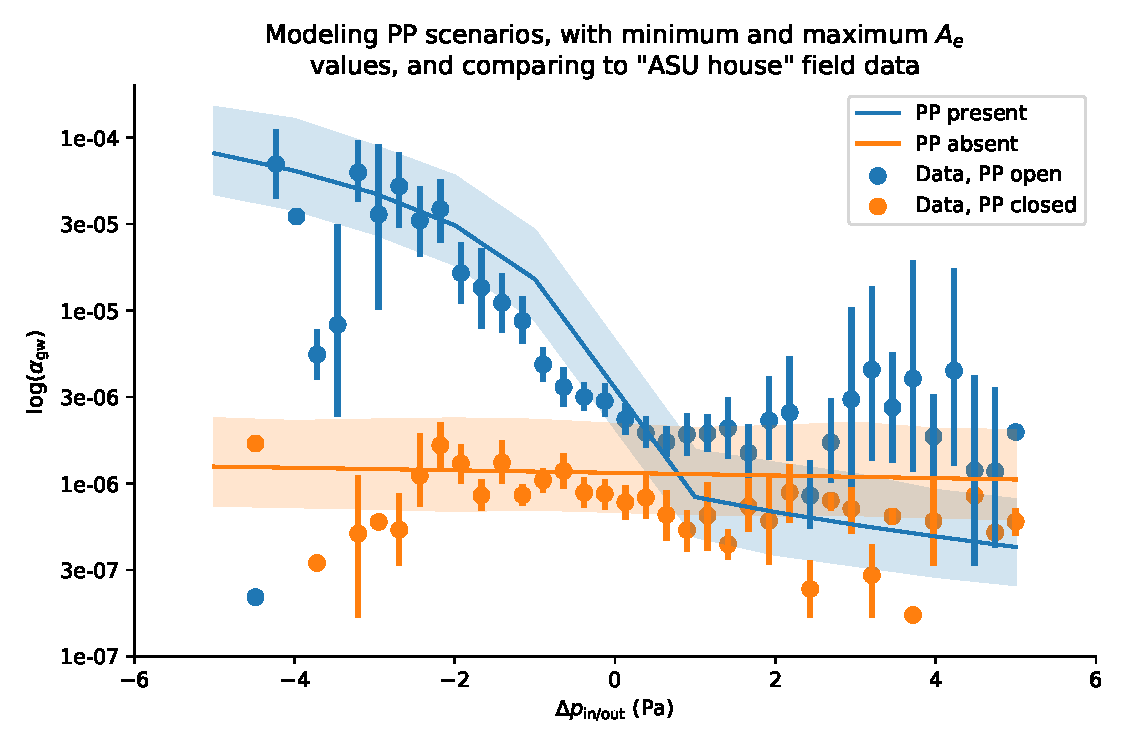
\includegraphics[width=\textwidth]{land_drain_scenarios_fluctuating_ae.pdf}
\end{figure}

% INTRODUCE THE FIGURE
To predict the variability of $\alpha_\mathrm{gw}$ for a given pressure, we use the minimum and maximum $A_e$ values observed at the ASU site (0.06 and 3.38 per hour respectively), and calculate $\alpha_\mathrm{gw}$ over the same range of $p_\mathrm{in/out}$ values.
This gives the range of values that $\alpha_\mathrm{gw}$ may fluctuate over for a given $p_\mathrm{in/out}$.
Using this method, the analysis in Figure \ref{fig:land_drain_scenarios_constant_ae} is repeated, i.e. that the cases when the preferential pathways is open and closed respectively are considered.
The result of this analysis can be seen in Figure \ref{fig:land_drain_scenarios_fluctuating_ae}, where this range of $\alpha_\mathrm{gw}$ is represented by the shaded areas, and the solid line is the predicted $\alpha_\mathrm{gw}$ when $A_e$ assumes the mean value of 0.50 per hour.
Data from ASU is binned in 40 evenly spaced bins, where the dot represents the mean value, and the error bars represent one standard deviation.

The trends in Figure \ref{fig:land_drain_scenarios_fluctuating_ae} are the same as in Figure \ref{fig:land_drain_scenarios_constant_ae}, but it is clear that much more variability is accounted for, especially considering the majority of datapoints were recorded between -3 and 3 Pa (the bins are evenly spaced, not evenly sized).
More e


% New PP simulations with extreme Ae values for each pressure considered
% Now we capture most of the variability for open and closed
% Strong indicator that fluctating Ae is responsible for a significant portion of the variability
% Needs to be controlled better (hard)
% Or the span of values considered to give upper and lower limits on variability
% Use EPA handbook to estimate variability (pretty much can always be one OOM)
\end{comment}





% Ergodicity argument here

% This says nothing about at what speed or timescale change may occur
% We look at the difference between max/min across various timespans
% See that on daily to a week, absent a PP, little variability is expected
% => 24 hr average samples adequate
% => no need to sample more than a few days apart
% Across time, more of the extreme values of Ae and pressure have occured, kind of ergodically, giving rise to this increase in variability
% Remember p and Ae are more or less normally distributed, (Ae more skewed)
% => extreme values unlikely but do happen across time


\subsection{Attenuation To Subslab} % TODO: Improve title


% Problem with attenuation to subslab
% Spatial variability in subslab may be greater than temporal indoor variability
% ASU perfect example, here there is greater alpha_sb variability than c
% => May be more uncertain
% => False positive for indoor sources
% => But could also indicate presence of PP in subbase
% Much larger spatial variability in subbase with PP present than without
% (Show plot with 2-4 panes)
% 1./2. show ASU/Indianapolis alpha_sb
% 3./4. model alpha_sb distributions with and without PP



\begin{acknowledgement}
  This project was supported by grant ES-201502 from the Strategic Environmental Research and Development Program and Environmental Security Technology Certification Program (SERDP-ESTCP).
\end{acknowledgement}

\bibliography{library}

\end{document}
